% --------------------------------------------------
% DOCUMENT CLASS
% --------------------------------------------------

\documentclass[
thesis.tex
]{subfiles}

\begin{document}
	
	\newpage
	
	\subsection{New Keynesian Model}\label{sec:nk-model}

	The model is populated by four agents: 
	\begin{enumerate*}[label=(\arabic*)]
		\item a representative household,
		\item a continuum of firms producing intermediate goods,
		\item a firm producing a final good, and
		\item the monetary authority.
	\end{enumerate*}
	
	The representative household maximizes utility based on consumption and labor, subject to a budget constraint composed of wages, capital rental rates, and firm profits.
	
	The final-goods firm produces the final-good consumed by households: it aggregates all intermediate-goods produced by intermediate firms, operates under perfect competition and seeks to maximize profit subject to the bundle technology.
	
	Intermediate firms each produce a single intermediate good, all exhibiting imperfect substitution, thus operating in monopolistic competition. Intermediate-goods firms has two problems to solve: minimize costs subject to production level and choose an optimal price to maximize the intertemporal profit flow.
	
	Periodically, a portion of intermediate-goods firms have the opportunity to adjust prices, while others miss this chance, following to a \textcite{calvo_staggered_1983} rule. This mechanism generates nominal price rigidities, altering equilibrium relationships in the system. These rigidities lead to non-neutrality of money in the short term, as explained by \textcite[p.191]{costa_junior_understanding_2016}.
	
	The monetary authority determines the nominal interest rate in response to fluctuations in previous period's inflation and production, aiming to control price levels and growth, following a \textcite{taylor_discretion_1993} rule.
	
	Stochastic shocks will be present in the intermediate-goods firms' productivity and in the monetary policy.
	
	For regionalization of the model, an index will be used to differentiate the studied region from the rest of Brazil, resulting in separate households, intermediate- and final-goods firms for each region.
	
	Households will lack mobility between regions. The link connecting the two regions will be the final-goods.
	
	Then, equilibrium conditions of the system will be determined. Assuming the system tends toward long-term equilibrium, a steady state will be reached where variables cease to change. Thus, for a given $t \longrightarrow \infty$, we will have $\boldsymbol{X}t = \boldsymbol{X}{t+1} = \boldsymbol{X}_{ss} \implies \boldsymbol{\dot{X}} = 0$.\footnote{recall that: $\boldsymbol{\dot{X}} = \frac{\partial \boldsymbol{X}}{\partial t}$} Here, $\boldsymbol{X}$ denotes the vector of system variables and $ss$ indicates the steady state.
	
	After that, the log-linearization method proposed by \textcite{uhlig_toolkit_1999} will be employed to convert the system of equations into a linear system, so that this linear system can be solved by the program \dynare{}, which computes the solution and produces impulse-response graphs based on the stochastic shocks.
	
	% Sixth, we will gather macroeconomic and regional data for the period from 1995 (the start of the plan) to 2020, using data from the first twenty years to estimate model parameters. Subsequently, we will assess the model's fit to data from the last six years.
	
	% --------------------------------------------------
	% MODEL DIAGRAM
	% --------------------------------------------------
	
	\subsection*{Model Diagram}
	
	\begin{figure}[h!]
		\centering
		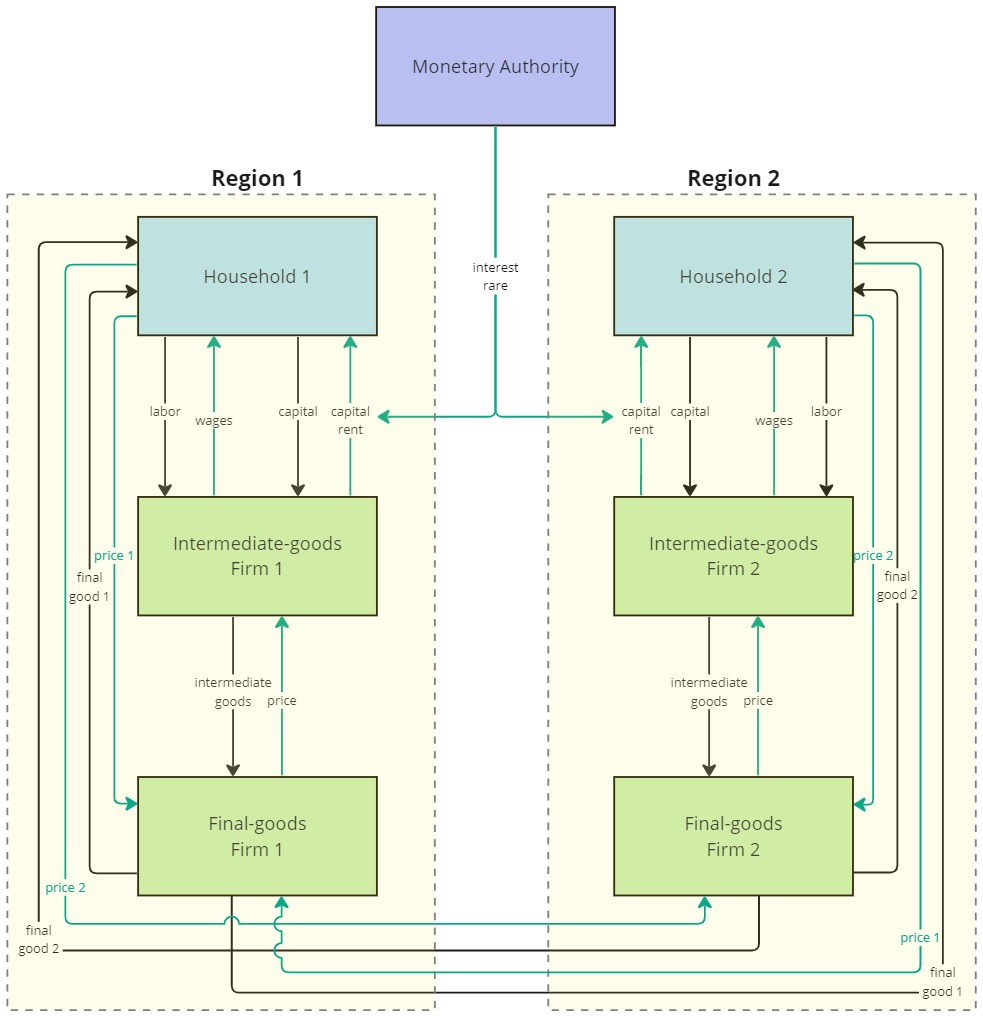
\includegraphics[width=\textwidth]{flowchart}
		\caption{Model Diagram}
		\label{fig:model-diagram}
	\end{figure}
	
	\newpage
	
	% --------------------------------------------------
	% HOUSEHOLD
	% --------------------------------------------------
	
	\subsubsection{Household}
	
	\subsubsection*{Utility Maximization Problem}
	
	% an \ac{uti} or \Ac{uti} or \acf{uti}
	
	Following the models presented by \textcite{costa_junior_understanding_2016} and \textcite{solis-garcia_ucb_2022}, the representative household problem is to maximize an intertemporal utility function $U$ with respect to consumption $C_t$ and labor $L_t$, subject to a budget constraint, a capital accumulation rule and the non-negativity of real variables:
	\begin{align}
		\label{eq:household-utility-function}
		\max_{C_t,L_t,K_{t+1}}: \quad & U(C_t,L_t) = \E \sum_{t=0}^{\infty} \beta^t \left(\frac{C_t^{1-\sigma}}{1-\sigma} - \phi \frac{L_t^{1+\varphi}}{1+\varphi} \right) \\
		\label{eq:household-budget-constraint}
		\st: \quad & P_t (C_t + I_t) = W_t L_t + R_t K_t + \Pi_t \\
		\label{eq:law-of-motion-for-capital}
		\quad & K_{t+1} = (1-\delta)K_t + I_t \\
		\quad & C_t,L_t,K_{t+1} \geq 0 \text{ ; $K_0$ given.} \nonumber
	\end{align}
	
	where $\E$ is the expectation operator, $\beta$ is the intertemporal discount factor, $\sigma$ is the relative risk aversion coefficient, $\phi$ is the labor relative weight in utility, $\varphi$ is the marginal disutility of labor supply. In the budget constraint, $P_t$ is the price level, $I_t$ is the investment, $W_t$ is the wage level, $K_t$ is the capital stock, $R_t$ is the return on capital, and $\Pi_t$ is the firm profit. In the capital accumulation rule, $\delta$ is the capital depreciation rate.
	
	Isolate $I_t$ in \ref{eq:law-of-motion-for-capital} and substitute in \ref{eq:household-budget-constraint}:
	\begin{align}
		\tag{\ref{eq:law-of-motion-for-capital}}
		& K_{t+1} = (1-\delta)K_t + I_t \implies I_t = K_{t+1} - (1-\delta)K_t \\
		\tag{\ref{eq:household-budget-constraint}}
		& P_t (C_t + I_t) = W_t L_t + R_t K_t + \Pi_t \implies \\
		\label{eq:household-budget-constraint-2}
		& P_t (C_t + K_{t+1} - (1-\delta)K_t) = W_t L_t + R_t K_t + \Pi_t
	\end{align}
	
	\subsubsection*{Lagrangian}
	
	The maximization problem with restriction can be transformed in one without restriction using the Lagrangian function $\mathcal{L}$ with \ref{eq:household-utility-function} and \ref{eq:household-budget-constraint-2}:
	\begin{multline}
		\label{eq:household-lagrangian}
		\mathcal{L} = \mathbb{E}_t \sum_{t=0}^{\infty} \beta^t 
		\left\{ \left( \frac{C_t^{1-\sigma}}{1-\sigma} - \phi \frac{L_t^{1+\varphi}}{1+\varphi} \right) - \right.
		\\
		\left. -\mu_t \Bigr[ P_t (C_t + K_{t+1} - (1-\delta) K_t) - (W_t L_t + R_t K_t + \Pi_t) \Bigl] \right\}
	\end{multline}
	
	\subsubsection*{First Order Conditions}
	
	The first order conditions with respect to $C_t$, $L_t$, $K_{t+1}$ and $\mu_t$ are:
	\begin{align}
		C_t: \quad & C_t^{-\sigma} -\mu_t P_t = 0 \implies \mu_t = \frac{C_t^{-\sigma}}{P_t} \label{eq:household-FOC-Ct} \\
		L_t: \quad & -\phi L_t^{\varphi} +\mu_t W_t = 0 \implies \mu_t = \frac{\phi L_t^{\varphi}}{W_t} \label{eq:household-FOC-Lt} \\
		\begin{split}
			K_{t+1}: \quad & -\mu_t P_t +\beta \mathbb{E}_t \mu_{t+1} [(1-\delta) P_{t+1} + R_{t+1}] = 0 \implies \\ & \qquad \mu_t P_t = \beta \mathbb{E}_t \mu_{t+1} [(1-\delta) P_{t+1} + R_{t+1}]
		\end{split} \label{eq:household-FOC-Kt} \\
		\mu_t: \quad & P_t (C_t + K_{t+1} - (1-\delta)K_t) = W_t L_t + R_t K_t + \Pi_t \tag{\ref{eq:household-budget-constraint-2}}
	\end{align}
	
	\subsubsection*{Solutions}
	
	Match equations \ref{eq:household-FOC-Ct} and \ref{eq:household-FOC-Lt}:
	\begin{align}
		\label{eq:household-labor-supply}
		\frac{C_t^{-\sigma}}{P_t} = \frac{\phi L_t^{\varphi}}{W_t} \implies 
		\frac{\phi L_t^{\varphi}}{C_t^{-\sigma}} = \frac{W_t}{P_t}
	\end{align}
	
	Equation \ref{eq:household-labor-supply} is the Household Labor Supply and shows that the marginal rate of substitution (MRS) of labor for consumption is equal to the real wage, which is the relative price between labor and goods.
	
	Substitute $\mu_t$ and $\mu_{t+1}$ from equation \ref{eq:household-FOC-Ct} in \ref{eq:household-FOC-Kt}:
	\begin{alignat}{2}
		\mu_t P_t & = \beta \mathbb{E}_t \mu_{t+1} [(1-\delta) P_{t+1} + R_{t+1}] \quad &\implies \nonumber \\
		\frac{C_t^{-\sigma}}{P_t} P_t & = \beta \mathbb{E}_t \frac{C_{t+1}^{-\sigma}}{P_{t+1}} [(1-\delta) P_{t+1} + R_{t+1}] &\implies \nonumber \\
		\left( \frac{\mathbb{E}_t C_{t+1}}{C_t} \right)^\sigma & = \beta \left[ (1-\delta) + \mathbb{E}_t \left(\frac{R_{t+1}}{P_{t+1}}\right) \right] \label{eq:household-euler-equation}
	\end{alignat}
	
	Equation \ref{eq:household-euler-equation} is the Household Euler equation.
	
	% --------------------------------------------------
	% FIRMS
	% --------------------------------------------------
	
	\subsection*{Firms}
	
	Consider two types of firms: 
	\begin{enumerate*}[label=(\arabic*)]
		\item a continuum of intermediate-good firms, which operate in monopolistic competition and each produce one variety with imperfect substitution level between each other and
		
		\item the final-good firm, which aggregates all the varieties into a final bundle and operates in perfect competition.
	\end{enumerate*}
	
	% --------------------------------------------------
	% FINAL-GOOD FIRM
	% --------------------------------------------------
	
	\subsubsection{Final-Good Firm}
	
	\subsubsection*{Profit Maximization Problem}
	
	The role of the final-good firm is to aggregate all the varieties produced by the intermediate-good firms, so that the representative consumer can buy only one good $Y_t$, the bundle good. The final-good firm problem is to maximize its profit, considering that its output is the bundle $Y_t$ formed by the continuum of intermediate goods $Y_{jt}$, where $j \in [0,1]$ and $\psi$ is the elasticity of substitution between intermediate goods:
	\begin{align}
		\label{eq:final-good-firm-max-problem}
		\max_{Y_{jt}}: &\quad \Pi_t = P_t Y_t - \int_{0}^{1} P_{jt} Y_{jt} \dif j\\
		\label{eq:final-good-firm-bundle-rule}
		\st: & \quad Y_t = \left( \int_{0}^{1} Y_{jt}^{\frac{\psi-1}{\psi}} \dif j \right)^{\frac{\psi}{\psi-1}}
	\end{align}
	
	Substitute \ref{eq:final-good-firm-bundle-rule} in \ref{eq:final-good-firm-max-problem}:
	\begin{align}
		\label{eq:final-good-firm-max-problem-2}
		\max_{Y_{jt}}: & \quad \Pi_t = P_t \left( \int_{0}^{1} Y_{jt}^{\frac{\psi-1}{\psi}} \dif j \right)^{\frac{\psi}{\psi-1}} - \int_{0}^{1} P_{jt} Y_{jt} \dif j
	\end{align}
	
	\subsubsection*{First Order Condition and Solutions}
	
	The first order condition is:
	\begin{align}
		Y_{jt}:\quad & P_t \left( \frac{\psi}{\psi-1} \right) \left( \int_{0}^{1} Y_{jt}^{\frac{\psi-1}{\psi}} \dif j \right)^{\frac{\psi}{\psi-1}-1} \left( \frac{\psi-1}{\psi} \right) Y_{jt}^{\frac{\psi-1}{\psi}-1} - P_{jt} = 0 \implies \nonumber \\
		\label{eq:final-good-firm-FOC}
		& Y_{jt} = Y_t \left( \frac{P_t}{P_{jt}} \right)^{\psi}
	\end{align}
	
	Equation \ref{eq:final-good-firm-FOC} shows that the demand for variety $j$ depends on its relative price. 
	
	Substitute \ref{eq:final-good-firm-FOC} in \ref{eq:final-good-firm-bundle-rule}:
	\begin{alignat}{2}
		Y_t & = \left( \int_{0}^{1} Y_{jt}^{\frac{\psi-1}{\psi}} \dif j \right)^{\frac{\psi}{\psi-1}} &\implies \nonumber \\
		Y_t & = \left( \int_{0}^{1} \left[ Y_t \left( \frac{P_t}{P_{jt}} \right)^{\psi} \right]^{\frac{\psi-1}{\psi}} \dif j \right)^{\frac{\psi}{\psi-1}} \quad &\implies \nonumber \\
		P_t & = \left[ \int_{0}^{1} P_{jt}^{1-\psi} \dif j \right]^{\frac{1}{1-\psi}} \label{eq:final-good-firm-markup}
	\end{alignat}
	
	Equation \ref{eq:final-good-firm-markup} is the final-good firm's markup.
	
	% --------------------------------------------------
	% INTERMEDIATE-GOOD FIRM
	% --------------------------------------------------
	
	\subsubsection{Intermediate-Good Firms}
	
	\subsubsection*{Cost Minimization Problem}
	
	The intermediate-good firms, denoted by $j \in [0,1]$, produce varieties of a representative good with a certain level of substitutability. Each of these firms has to choose capital $K_{jt}$ and labor $N_{jt}$ to minimize production costs, subject to a technology rule.
	\begin{align}
		\label{eq:int-good-firm-total-cost}
		\min_{K_{jt}, L_{jt}}: \quad & R_t K_{jt} + W_t L_{jt} \\
		\label{eq:int-good-firm-production-function}
		\st: \quad & Y_{jt} = Z_{At} K_{jt}^\alpha L_{jt}^{1-\alpha}
	\end{align}
	
	where $Y_{jt}$ is the output obtained by the production technology level $Z_{At}$\footnotemark{} that transforms capital $K_{jt}$ and labor $L_{jt}$ in proportions $\alpha$ and $(1-\alpha)$, respectively, into intermediate goods.
	
	\footnotetext{the production technology level $Z_{At}$ will be submitted to a productivity shock, detailed in section \ref{sec:productivity shock}.}
	
	\subsubsection*{Lagrangian}
	
	Applying the Lagrangian:
	\begin{align}
		\label{eq:int-good-firm-lagrangian}
		\mathcal{L} = (R_t K_{jt} + W_t L_{jt}) - \Lambda_t (Z_{At} K_{jt}^\alpha L_{jt}^{1-\alpha} - Y_{jt})
	\end{align}
	
	where the Lagrangian multiplier $\Lambda_t$ is the marginal cost\footnote{see Lemma \ref{lemma:marginal-cost}}.
	
	\subsubsection*{First Order Conditions}
	
	The first-order conditions are:
	\begin{alignat}{2}
		K_{jt}: \quad & R_t - \Lambda_t Z_{At} \alpha K_{jt}^{\alpha-1} L_{jt}^{1-\alpha} = 0 &&\implies K_{jt} = \alpha Y_{jt} \frac{\Lambda_t}{R_t} \label{eq:int-good-firm-FOC-Kt} \\
		L_{jt}: \quad & W_t - \Lambda_t Z_{At} K_{jt}^\alpha (1-\alpha) L_{jt}^{-\alpha} = 0 \quad &&\implies L_{jt} = (1-\alpha) Y_{jt} \frac{\Lambda_t}{W_t} \label{eq:int-good-firm-FOC-Lt} \\
		\Lambda_t: \quad & Y_{jt} = Z_{At} K_{jt}^\alpha L_{jt}^{1-\alpha} \tag{\ref{eq:int-good-firm-production-function}}
	\end{alignat}
	
	\subsubsection*{Solutions}
	
	Divide equation \ref{eq:int-good-firm-FOC-Kt} by \ref{eq:int-good-firm-FOC-Lt}:
	\begin{align}
		\frac{K_{jt}}{L_{jt}} = \frac{\alpha Y_{jt} \Lambda_t /R_t}{(1-\alpha) Y_{jt} \Lambda_t /W_t} \implies
		\frac{K_{jt}}{L_{jt}} = \left( \frac{\alpha}{1-\alpha} \right) \frac{W_t}{R_t} \label{eq:int-good-firm-TMRS}
	\end{align}
	
	Equation \ref{eq:int-good-firm-TMRS} demonstrates the relationship between the technical marginal rate of substitution (TMRS) and the economical marginal rate of substitution (EMRS). 
	
	Substitute $L_{jt}$ from equation \ref{eq:int-good-firm-TMRS} in \ref{eq:int-good-firm-production-function}:
	\begin{alignat}{2}
		Y_{jt} & = Z_{At} K_{jt}^\alpha L_{jt}^{1-\alpha} &\implies \nonumber \\
		Y_{jt} & = Z_{At} K_{jt}^\alpha \left[ \left( \frac{1-\alpha}{\alpha} \right) \frac{R_t K_{jt}}{W_t} \right]^{1-\alpha} &\implies \nonumber \\
		K_{jt} & = \frac{Y_{jt}}{Z_{At}} \left[ \left( \frac{\alpha}{1-\alpha} \right) \frac{W_t}{R_t}\right]^{1-\alpha} \label{eq:int-good-firm-Kt-demand}
	\end{alignat}
	
	Equation \ref{eq:int-good-firm-Kt-demand} is the intermediate-good firm demand for capital. 
	
	Substitute \ref{eq:int-good-firm-Kt-demand} in \ref{eq:int-good-firm-TMRS}:
	\begin{alignat}{2}
		L_{jt} & = \left( \frac{1-\alpha}{\alpha} \right) \frac{R_t K_{jt}}{W_t} &\implies \nonumber \\
		L_{jt} & = \left( \frac{1-\alpha}{\alpha} \right) \frac{R_t}{W_t} \frac{Y_{jt}}{Z_{At}} \left[ \left( \frac{\alpha}{1-\alpha} \right) \frac{W_t}{R_t}\right]^{1-\alpha} &\implies \nonumber \\
		L_{jt} & = \frac{Y_{jt}}{Z_{At}} \left[ \left( \frac{\alpha}{1-\alpha} \right) \frac{W_t}{R_t}\right]^{-\alpha} \label{eq:int-good-firm-Lt-demand}
	\end{alignat}
	
	Equation \ref{eq:int-good-firm-Lt-demand} is the intermediate-good firm demand for labor.
	
	\subsubsection*{Total and Marginal Costs}
	
	Calculate the total cost using \ref{eq:int-good-firm-Kt-demand} and \ref{eq:int-good-firm-Lt-demand}:
	\begin{alignat}{2}
		TC_{jt} & = W_t L_{jt} + R_t K_{jt} &\implies \nonumber \\
		TC_{jt} & = W_t \frac{Y_{jt}}{Z_{At}} \left[ \left( \frac{\alpha}{1-\alpha} \right) \frac{W_t}{R_t} \right]^{-\alpha} + R_t \frac{Y_{jt}}{Z_{At}} \left[ \left( \frac{\alpha}{1-\alpha} \right) \frac{W_t}{R_t} \right]^{1-\alpha} &\implies \nonumber \\
		TC_{jt} & = \frac{Y_{jt}}{Z_{At}} \left( \frac{R_t}{\alpha} \right)^{\alpha} \left( \frac{W_t}{1-\alpha} \right)^{1-\alpha} \label{eq:int-good-firm-TC}
	\end{alignat}
	
	%%%%%
	
	Calculate the marginal cost using \ref{eq:int-good-firm-TC}: 
	\begin{align}
		\label{eq:int-good-firm-MC}
		\Lambda_{jt} & = \frac{\partial TC_{jt}}{\partial Y_{jt}}
		\implies 
		\Lambda_{jt} = \frac{1}{Z_{At}} \left( \frac{R_t}{\alpha} \right)^{\alpha} \left( \frac{W_t}{1-\alpha} \right)^{1-\alpha}
	\end{align}
	
	The marginal cost depends on the technological level $Z_{At}$, the nominal interest rate $R_t$ and the nominal wage level $W_t$, which are the same for all intermediate-good firms, and because of that, the index $j$ may be dropped:
	\begin{align}
		\label{eq:int-good-firm-MC-2}
		\Lambda_t = \frac{1}{Z_{At}} \left( \frac{R_t}{\alpha} \right)^{\alpha} \left( \frac{W_t}{1-\alpha} \right)^{1-\alpha}
	\end{align}
	
	notice that:
	\begin{align}
		\label{eq:int-good-firm-TC-MC}
		\Lambda_t = \frac{TC_{jt}}{Y_{jt}} \implies 
		TC_{jt} = \Lambda_t Y_{jt}
	\end{align}
	
	% --------------------------------------------------
	% CALVO RULE
	% --------------------------------------------------
	
	\subsubsection*{Optimal Price Problem}
	
	Consider an economy with price stickiness, following the Calvo Rule \cite{calvo_staggered_1983}: each firm has a probability $(0 < \theta < 1)$ of keeping its price in the next period ($P_{j,t+1} = P_{j,t}$), and a probability of $(1 - \theta)$ of setting a new optimal price $P_{j,t}^\ast$ that maximizes its profits. Therefore, each firm must take this uncertainty into account when deciding the optimal price: the intertemporal profit flow, given the nominal interest rate $R_t$ of each period, is calculated considering the probability $\theta$ of keeping the previous price.
	\begin{align}
		\max_{P_{jt}}: & \quad \E \sum_{s=0}^{\infty} \left\{ \frac{ \theta^s \left[ P_{jt} Y_{j,t+s} - TC_{j,t+s} \right] }{\prod_{k=0}^{s-1}(1+R_{t+k})} \right\} \label{eq:int-good-firm-optimal-price-problem} \\
		\st: & \quad Y_{jt} = Y_t \left( \frac{P_t}{P_{jt}} \right)^{\psi} \tag{\ref{eq:final-good-firm-FOC}}
	\end{align}
	
	%%%%%
	
	Substitute \ref{eq:int-good-firm-TC-MC} in \ref{eq:int-good-firm-optimal-price-problem}:
	\begin{align}
		\label{eq:int-good-firm-optimal-price-problem-2}
		\max_{P_{jt}}: & \quad \E \sum_{s=0}^{\infty} \left\{ \frac{\theta^s \big[ P_{jt} Y_{j,t+s} - \Lambda_{t+s} Y_{j,t+s} \big]}{\prod_{k=0}^{s-1}(1+R_{t+k})} \right\}
	\end{align}
	
	Substitute \ref{eq:final-good-firm-FOC} in \ref{eq:int-good-firm-optimal-price-problem-2} and rearrange the variables:
	\begin{align}
		\max_{P_{jt}}: & \quad \E \sum_{s=0}^{\infty} \left\{ \frac{\theta^s \left[ P_{jt} Y_{t+s} \left( \frac{P_{t+s}}{P_{jt}} \right)^{\psi} - \Lambda_{t+s} Y_{t+s} \left( \frac{P_{t+s}}{P_{jt}} \right)^{\psi} \right] }{\prod_{k=0}^{s-1}(1+R_{t+k})} \right\} \implies \nonumber 
		\\
		\max_{P_{jt}}: & \quad \E \sum_{s=0}^{\infty} \left\{ \frac{\theta^s \left[ P_{jt}^{1-\psi} P_{t+s}^{\psi} Y_{t+s} - P_{jt}^{-\psi} P_{t+s}^{\psi} Y_{t+s} \Lambda_{t+s} \right] }{\prod_{k=0}^{s-1}(1+R_{t+k})} \right\} \nonumber
	\end{align}
	
	%%%%%
	
	\subsubsection*{First Order Condition}
	
	The first order condition with respect to $P_{jt}$ is:
	\begin{align}
		& \quad \E \sum_{s=0}^{\infty} \left\{ \frac{\theta^s \left[ (1-\psi) P_{jt}^{-\psi} P_{t+s}^{\psi} Y_{t+s} - (-\psi) P_{jt}^{-\psi-1} P_{t+s}^{\psi} Y_{t+s} \Lambda_{t+s} \right] }{\prod_{k=0}^{s-1}(1+R_{t+k})} \right\} = 0 \nonumber
	\end{align}
	
	%%%%%
	
	Separate the summations and rearrange the variables:
	\begin{align}
		\label{eq:int-good-firm-optimal-price-FOC}
		& \E \sum_{s=0}^{\infty} \left\{ \frac{\theta^s (\psi-1) \left( \frac{P_{t+s}} {P_{jt}} \right)^{\psi} Y_{t+s}} {\prod_{k=0}^{s-1} (1+R_{t+k})} \right\} = \E \sum_{s=0}^{\infty} \left\{ \frac{\theta^s \psi P_{jt}^{-1} \left( \frac{P_{t+s}} {P_{jt}} \right)^{\psi} Y_{t+s} \Lambda_{t+s} }{\prod_{k=0}^{s-1}(1+R_{t+k})} \right\}
	\end{align}
	
	%%%%%
	
	Substitute \ref{eq:final-good-firm-FOC} in \ref{eq:int-good-firm-optimal-price-FOC}:
	\begin{alignat}{2}
		\E \sum_{s=0}^{\infty} \Bigg\{ \frac{\theta^s (\psi-1) Y_{j,t+s}}{\prod_{k=0}^{s-1}(1+R_{t+k})} \Bigg\} &= \E \sum_{s=0}^{\infty} \Bigg\{ \frac{\theta^s \psi P_{jt}^{-1} Y_{j,t+s} \Lambda_{t+s}}{\prod_{k=0}^{s-1}(1+R_{t+k})}  \Bigg\} &\implies \nonumber \\
		(\psi-1) \E \sum_{s=0}^{\infty} \Bigg\{ \frac{\theta^s Y_{j,t+s}}{\prod_{k=0}^{s-1}(1+R_{t+k})} \Bigg\} &= \psi P_{jt}^{-1} \E \sum_{s=0}^{\infty} \Bigg\{ \frac{\theta^s Y_{j,t+s} \Lambda_{t+s}}{\prod_{k=0}^{s-1}(1+R_{t+k})}  \Bigg\} &\implies \nonumber \\
		P_{jt} \E \sum_{s=0}^{\infty} \Bigg\{ \frac{\theta^s Y_{j,t+s}}{\prod_{k=0}^{s-1}(1+R_{t+k})} \Bigg\} &= \frac{\psi}{\psi-1} \E \sum_{s=0}^{\infty} \Bigg\{ \frac{\theta^s Y_{j,t+s} \Lambda_{t+s}}{\prod_{k=0}^{s-1}(1+R_{t+k})}  \Bigg\} &\implies \nonumber
	\end{alignat}
	
	\vspace*{-1cm}
	
	\begin{align}
		\label{eq:int-good-firm-optimal-price-FOC-2}
		P_{jt}^\ast &= 
		\frac{\psi}{\psi-1} \cdot
		\frac{
			\E \sum_{s=0}^{\infty} \left\{ 
			\theta^s Y_{j,t+s} \Lambda_{t+s} / \prod_{k=0}^{s-1}(1+R_{t+k}) \right\} } {\E \sum_{s=0}^{\infty} \left\{
			\theta^s Y_{j,t+s} / \prod_{k=0}^{s-1}(1+R_{t+k}) \right\}}
	\end{align}
	
	% as firmas que maximizam em dado período, escolherão o mesmo preço, P novo i,t = P (ot) t (Walsh 2003, pág. 235).
	
	Equation \ref{eq:int-good-firm-optimal-price-FOC-2} represents the optimal price that firm $j$ will choose. Since all firms that are able to choose will opt for the highest possible price, they will all select the same price. As a result, the index $j$ can be omitted:
	\begin{align}
		\label{eq:int-good-firm-optimal-price-FOC-3}
		P_t^\ast &= 
		\frac{\psi}{\psi-1} \cdot
		\frac{
			\E \sum_{s=0}^{\infty} \left\{ 
			\theta^s Y_{j,t+s} \Lambda_{t+s} / \prod_{k=0}^{s-1}(1+R_{t+k}) \right\} } {\E \sum_{s=0}^{\infty} \left\{
			\theta^s Y_{j,t+s} / \prod_{k=0}^{s-1}(1+R_{t+k}) \right\}}
	\end{align}
	
	% --------------------------------------------------
	% FINAL-GOOD FIRM, PART II
	% --------------------------------------------------
	
	\subsubsection{Final-Good Firm, part II}
	
	The process of fixing prices is random: in each period, $\theta$ firms will maintain the price from the previous period, while $(1-\theta)$ firms will choose a new optimal price. The price level for each period will be a composition of these two prices. Use this information in \ref{eq:final-good-firm-markup} to determine the aggregate price level:
	\begin{align}
		P_t & = \left[ \int_{0}^{\theta} P_{t-1}^{1-\psi} \dif j + \int_{\theta}^{1} P_t^{\ast 1-\psi} \dif j \right]^{\frac{1}{1-\psi}}  \implies \nonumber \\
		P_t & = \left[ \theta P_{t-1}^{1-\psi} + (1-\theta) P_t^{\ast 1-\psi} \right]^\frac{1}{1-\psi} \label{eq:general-price-level}
	\end{align}
	
	Equation \ref{eq:general-price-level} is the aggregate price level.
	
	% --------------------------------------------------
	% MONETARY AUTHORITY
	% --------------------------------------------------
	
	\subsubsection{Monetary Authority}
	
	The objective of the monetary authority is to conduct the economy to price stability and economic growth, using a Taylor rule \cite{taylor_discretion_1993} to determine the nominal interest rate:
	\begin{align}
		\label{eq:monetary-policy}
		\frac{R_t}{R} =
		\left( \frac{R_{t-1}}{R} \right)^{\gamma_R}  \left[
		\left( \frac{\pi_t}{\pi} \right)^{\gamma_\pi}
		\left( \frac{Y_t}{Y} \right)^{\gamma_Y} \right]^{1-\gamma_R} Z_{Mt}
	\end{align}
	
	where $\pi_t$ is the gross inflation rate, defined by:
	\begin{align}
		\pi_t = \frac{P_t}{P_{t-1}}
		\label{eq:gross-inflation-rate}
	\end{align}
	
	and $R, \pi, Y$ are the variables in steady state, $\gamma_R$ is the smoothing parameter for the interest rate $R_t$, while $\gamma_\pi$ and $\gamma_Y$ are the interest-rate sensitivities in relation to inflation and product, respectively and $Z_{Mt}$ is the monetary shock\footnote{for the monetary shock definition, see section \ref{sec:monetary shock}.}.
	
	% --------------------------------------------------
	% STOCHASTIC SHOCKS
	% --------------------------------------------------
	
	\subsubsection{Stochastic Shocks}\label{sec:stochastic-shocks}
	
	\subsubsection*{Productivity Shock} \label{sec:productivity shock}
	
	The production technology level $Z_{At}$ will be submitted to a productivity shock defined by a first-order autoregressive process $AR(1)$:
	\begin{align}
		\ln{Z_{At}} = (1-\rho_A)\ln{Z_A} + \rho_A\ln{Z_{A,t-1}} + \varepsilon_{At} \label{eq:productivity-shock}
	\end{align}
	
	where $\rho_A \in [0,1]$ is the autoregressive parameter and $\varepsilon_{At} \sim \mathscr{N}(0,\sigma_A)$.
	
	\subsubsection*{Monetary Shock} \label{sec:monetary shock}
	
	The monetary policy will also be submitted to a shock, through the variable $Z_{Mt}$, defined by a first-order autoregressive process $AR(1)$:
	\begin{align}
		\ln{Z_{Mt}} = (1-\rho_M)\ln{Z_{M}} + \rho_M\ln{Z_{M,t-1}} + \varepsilon_{Mt} \label{eq:monetary-shock}
	\end{align}
	
	where $\rho_M \in [0,1]$ and $\varepsilon_{Mt} \sim \mathscr{N}(0,\sigma_M)$.
	
	% --------------------------------------------------
	% EQUILIBRIUM CONDITIONS
	% --------------------------------------------------
	
	\subsubsection{Equilibrium Conditions}
	
	% removed from the household solution set: I_t^\ast, 
	
	A Competitive Equilibrium consists of sequences of prices $\{P_t^\ast, R_t^\ast, W_t^\ast\}$, allocations for households $\mathbfscr{A}_H \coloneq \{C_t^\ast, L_t^\ast, K_{t+1}^\ast\}$ and for firms $\mathbfscr{A}_F \coloneq \{K_{jt}^\ast, L_{jt}^\ast, Y_{jt}^\ast, Y_t^\ast\}$. In such an equilibrium, given the set of exogenous variables $\{K_0, Z_{At}, Z_{Mt}\}$, the elements in $\mathbfscr{A}_H$ solve the household problem, while the elements in $\mathbfscr{A}_F$ solve the firms' problems, and the markets for goods and labor clear:
	\begin{align}
		Y_t &= C_t + I_t \label{eq:market-clearing-condition} \\
		L_t &= \int_{0}^{1} L_{jt} \dif j \label{eq:market-clearing-condition-2}
	\end{align}
	
	%\newpage
	
	% --------------------------------------------------
	% MODEL STRUCTURE
	% --------------------------------------------------
	
	\subsubsection{Model Structure}
	
	The model is composed of the preview solutions, forming a square system of 16 variables and 16 equations, summarized as follows:
	
	{\singlespacing
		
		\begin{itemize}
			\item Variables (16):
			
			\begin{itemize}
				\item from the household problem: $C_t, L_t, K_{t+1}$;
				\item from the final-good firm problem: $Y_{jt}, P_t$;
				\item from the intermediate-good firm problems: $K_{jt}, L_{jt}, P_t^\ast$;
				\item from the market clearing condition: $Y_t, I_t$;
				\item prices: $W_t, R_t, \Lambda_t, \pi_t$;
				\item shocks: $Z_{At}, Z_{Mt}$.
			\end{itemize}
			\item Equations (16):
			
			\begin{enumerate}
				\item Labor Supply:
				\begin{align}
					\frac{\phi L_t^{\varphi}}{C_t^{-\sigma}} = \frac{W_t}{P_t}
					\tag{\ref{eq:household-labor-supply}}
				\end{align}
				
				\item Household Euler Equation:
				\begin{align}
					\left( \frac{\mathbb{E}_t C_{t+1}}{C_t} \right)^\sigma = \beta \left[ (1-\delta) + \mathbb{E}_t \left(\frac{R_{t+1}}{P_{t+1}}\right) \right]
					\tag{\ref{eq:household-euler-equation}}
				\end{align}
				
				\item Budget Constraint: 
				\begin{align}
					P_t (C_t + I_t) = W_t L_t + R_t K_t + \Pi_t
					\tag{\ref{eq:household-budget-constraint}}
				\end{align}
				
				\item Law of Motion for Capital:
				\begin{align}
					K_{t+1} = (1-\delta)K_t + I_t
					\tag{\ref{eq:law-of-motion-for-capital}}
				\end{align}
				
				\item Bundle Technology:
				\begin{align}
					Y_t = \left( \int_{0}^{1} Y_{jt}^{\frac{\psi-1}{\psi}} \dif j \right)^{\frac{\psi}{\psi-1}}
					\tag{\ref{eq:final-good-firm-bundle-rule}}
				\end{align}
				
				\item General Price Level:
				\begin{align}
					P_t = \left[ \theta P_{t-1}^{1-\psi} + (1-\theta) P_t^{\ast 1-\psi} \right]^\frac{1}{1-\psi}
					\tag{\ref{eq:general-price-level}}
				\end{align}
				
				\item Capital Demand:
				\begin{align}
					K_{jt} = \alpha Y_{jt} \frac{\Lambda_t}{R_t}
					\tag{\ref{eq:int-good-firm-FOC-Kt}}
				\end{align}
				
				\item Labor Demand:
				\begin{align}
					L_{jt} = (1-\alpha) Y_{jt} \frac{\Lambda_t}{W_t}
					\tag{\ref{eq:int-good-firm-FOC-Lt}}
				\end{align}
				
				% \item Marginal Rate of Substitution of Factors (\ref{eq:int-good-firm-TMRS}):
				% \[ \frac{K_{jt}}{L_{jt}} = \left( \frac{\alpha}{1-\alpha} \right) \frac{W_t}{R_t} \]
				
				\item Marginal Cost:
				\begin{align}
					\Lambda_t = \frac{1}{Z_{At}} \left( \frac{R_t}{\alpha} \right)^{\alpha} \left( \frac{W_t}{1-\alpha} \right)^{1-\alpha}
					\tag{\ref{eq:int-good-firm-MC-2}}
				\end{align}
				
				\item Production Function:
				\begin{align}
					Y_{jt} = Z_{At} K_{jt}^\alpha L_{jt}^{1-\alpha}
					\tag{\ref{eq:int-good-firm-production-function}}
				\end{align}
				
				\item Optimal Price:
				\begin{align}
					P_t^\ast = \frac{\psi}{\psi-1} \cdot \frac{ \E \sum_{s=0}^{\infty} \left\{ \theta^s Y_{j,t+s} \Lambda_{t+s} / \prod_{k=0}^{s-1}(1+R_{t+k}) \right\} } {\E \sum_{s=0}^{\infty} \left\{ \theta^s Y_{j,t+s} / \prod_{k=0}^{s-1}(1 + R_{t+k}) \right\}} \tag{\ref{eq:int-good-firm-optimal-price-FOC-3}}
				\end{align}
				
				\item Market Clearing Condition:
				\begin{align}
					Y_t = C_t + I_t
					\tag{\ref{eq:market-clearing-condition}}
				\end{align}
				
				\item Monetary Policy:
				\begin{align}
					\frac{R_t}{R} = \left( 
					\frac{R_{t-1}}{R} \right)^{\gamma_R} \left[ \left(
					\frac{\pi_t}{\pi} \right)^{\gamma_\pi} \left( 
					\frac{Y_t}{Y} \right)^{\gamma_Y} \right]^{1-\gamma_R} Z_{Mt}
					\tag{\ref{eq:monetary-policy}}
				\end{align}
				
				\item Gross Inflation Rate:
				\begin{align}
					\pi_t = \frac{P_t}{P_{t-1}}
					\tag{\ref{eq:gross-inflation-rate}}
				\end{align}
				
				\item Productivity Shock:
				\begin{align}
					\ln{Z_{At}} = (1-\rho_A)\ln{Z_A} + \rho_A\ln{Z_{A,t-1}} + \varepsilon_{At}
					\tag{\ref{eq:productivity-shock}}
				\end{align}
				
				\item Monetary Shock:
				\begin{align}
					\ln{Z_{Mt}} = (1-\rho_M)\ln{Z_{M}} + \rho_M\ln{Z_{M,t-1}} + \varepsilon_{Mt}
					\tag{\ref{eq:monetary-shock}}
				\end{align}
				
			\end{enumerate}
			
		\end{itemize}
		
	} % \singlespacing
	
	%\newpage
	
	% --------------------------------------------------
	% STEADY STATE
	% --------------------------------------------------
	
	\subsubsection{Steady State}
	
	The steady state is defined by the constancy of the variables through time. For any given endogenous variable $X_t$, it is in steady state if $\mathbb{E}_t X_{t+1} = X_t = X_{t-1} = X_{ss}$ \cite[p.41]{costa_junior_understanding_2016}. For conciseness, the $ss$ index representing the steady state will be omitted, so that $X \coloneq X_{ss}$. The steady state of each equation of the model is:
	
	\begin{enumerate}
		\item Labor Supply:
		\begin{align}
			\label{eq:ss-household-labor-supply}
			\frac{\phi L_t^{\varphi}}{C_t^{-\sigma}} = \frac{W_t}{P_t} \implies
			\frac{\phi L^{\varphi}}{C^{-\sigma}} = \frac{W}{P}
		\end{align}
		
		\item Household Euler Equation: 
		\begin{align}
			\label{eq:ss-household-euler-equation}
			\left( \frac{\mathbb{E}_t C_{t+1}}{C_t} \right)^\sigma = \beta \left[ (1-\delta) + \mathbb{E}_t \left(\frac{R_{t+1}}{P_{t+1}}\right) \right] \implies 
			1 = \beta \left[ (1-\delta) + \frac{R}{P} \right]
		\end{align}
		
		\item Budget Constraint: 
		\begin{align}
			\label{eq:ss-household-budget-constraint}
			P_t (C_t + I_t) = W_t L_t + R_t K_t + \Pi_t \implies 
			P (C + I) = W L + R K + \Pi
		\end{align}
		
		\item Law of Motion for Capital:
		\begin{align}
			\label{eq:ss-law-of-motion-for-capital}
			K_{t+1} = (1-\delta)K_t + I_t \implies
			K = (1-\delta)K + I \implies I = \delta K
		\end{align}
		
		\item Bundle Technology:
		\begin{align}
			\label{eq:ss-final-good-firm-bundle-rule}
			Y_t = \left( \int_{0}^{1} Y_{jt}^{\frac{\psi-1}{\psi}} \dif j \right)^{\frac{\psi}{\psi-1}} \implies 
			Y = \left( \int_{0}^{1} Y_{j}^{\frac{\psi-1}{\psi}} \dif j \right)^{\frac{\psi}{\psi-1}}
		\end{align}
		
		\item General Price Level:
		\begin{alignat}{2}
			\label{eq:ss-general-price-level}
			P_t &= \left[ \theta P_{t-1}^{1-\psi} + (1-\theta) P_t^{\ast 1-\psi} \right]^\frac{1}{1-\psi} &&\implies \nonumber \\
			P^{1-\psi} &= \theta P^{1-\psi} + (1-\theta) P^{\ast 1-\psi} &&\implies \nonumber \\ 
			(1-\theta) P^{1-\psi} &= (1-\theta) P^{\ast 1-\psi} &&\implies P = P^\ast
		\end{alignat}
		
		\item Capital Demand:
		\begin{align}
			\label{eq:ss-int-good-firm-FOC-Kt}
			K_{jt} = \alpha Y_{jt} \frac{\Lambda_t}{R_t} \implies 
			K_{j} = \alpha Y{j} \frac{\Lambda}{R}
		\end{align}
		
		\item Labor Demand:
		\begin{align}
			\label{eq:ss-int-good-firm-FOC-Lt}
			L_{jt} = (1-\alpha) Y_{jt} \frac{\Lambda_t}{W_t} \implies 
			L_{j} = (1-\alpha) Y{j} \frac{\Lambda}{W}
		\end{align}
		
		% \item Marginal Rate of Substitution of Factors (\ref{eq:int-good-firm-TMRS}):
		% \[ \frac{K_{jt}}{L_{jt}} = \left( \frac{\alpha}{1-\alpha} \right) \frac{W_t}{R_t} \]
		
		\item Marginal Cost:
		\begin{align}
			\label{eq:ss-int-good-firm-MC-2}
			\Lambda_t = \frac{1}{Z_{At}} \left( \frac{R_t}{\alpha} \right)^{\alpha} \left( \frac{W_t}{1-\alpha} \right)^{1-\alpha} \implies
			\Lambda = \frac{1}{Z_{A}} \left( \frac{R}{\alpha} \right)^{\alpha} \left( \frac{W}{1-\alpha} \right)^{1-\alpha}
		\end{align}
		
		\item Production Technology:
		\begin{align}
			\label{eq:ss-int-good-firm-production-function}
			Y_{jt} = Z_{At} K_{jt}^\alpha L_{jt}^{1-\alpha} \implies 
			Y_{j} = Z_{A} K_{j}^\alpha L_{j}^{1-\alpha}
		\end{align}
		
		\item Optimal Price:
		\begin{alignat}{2}
			P_t^\ast &= \frac{\psi}{\psi-1} \cdot \frac{\E \sum_{s=0}^{\infty} \left\{\theta^s Y_{j,t+s} \Lambda_{t+s} / \prod_{k=0}^{s-1}(1+R_{t+k}) \right\}} {\E \sum_{s=0}^{\infty} \left\{ \theta^s Y_{j,t+s} / \prod_{k=0}^{s-1}(1+R_{t+k}) \right\}} &\implies \tag{\ref{eq:int-good-firm-optimal-price-FOC-3}} \\
			P^\ast &= \frac{\psi}{\psi-1} \cdot \frac{ Y_j \Lambda / [1-\theta(1-R)]} {Y_j / [1-\theta(1-R)]} &\implies \nonumber \\
			P^\ast &= \frac{\psi}{\psi-1} \Lambda \label{eq:ss-int-good-firm-optimal-price-FOC-3}
		\end{alignat}
		
		\item Market Clearing Condition:
		\begin{align}
			\label{eq:ss-market-clearing-condition}
			Y_t = C_t + I_t \implies Y = C + I
		\end{align}
		
		\item Monetary Policy:
		\begin{align}
			\label{eq:ss-monetary-policy}
			\frac{R_t}{R} =
			\left( \frac{R_{t-1}}{R} \right)^{\gamma_R}  \left[
			\left( \frac{\pi_t}{\pi} \right)^{\gamma_\pi}
			\left( \frac{Y_t}{Y} \right)^{\gamma_Y} \right]^{1-\gamma_R} Z_{Mt}
			\implies Z_{M} = 1
		\end{align}
		
		\item Gross Inflation Rate:
		\begin{align}
			\label{eq:ss-gross-inflation-rate}
			\pi_t = \frac{P_t}{P_{t-1}} \implies \pi = 1
		\end{align}
		
		\item Productivity Shock:
		\begin{alignat}{2}
			\ln{Z_{At}} &= (1-\rho_A)\ln{Z_A} + \rho_A\ln{Z_{A,t-1}} + \varepsilon_{At} \quad &\implies \nonumber \\
			\ln{Z_{A}} &= (1-\rho_A)\ln{Z_A} + \rho_A\ln{Z_{A}} + \varepsilon_{A} &\implies \nonumber \\
			\varepsilon_{A} &= 0 \label{eq:ss-productivity-shock}
		\end{alignat}
		
		\item Monetary Shock:
		\begin{alignat}{2}
			\ln{Z_{Mt}} &= (1-\rho_M)\ln{Z_{M}} + \rho_M\ln{Z_{M,t-1}} + \varepsilon_{Mt} \quad &\implies \nonumber \\
			\ln{Z_{M}} &= (1-\rho_M)\ln{Z_{M}} + \rho_M\ln{Z_{M}} + \varepsilon_{M} &\implies \nonumber \\
			\varepsilon_{M} &= 0 \label{eq:ss-monetary-shock}
		\end{alignat}
		
	\end{enumerate}
	
	% --------------------------------------------------
	% STEADY STATE SOLUTION
	% --------------------------------------------------
	
	\subsubsection{Variables in Steady State}
	
	% All endogenous prices $\{P, R, W, MC\}$ and quantities $\{C, I, Y, K, L\}$
	
	For the steady state solution, all endogenous variables will be determined with respect to the parameters. It's assumed that the productivity and the price level are normalized to one: $\left[ \begin{smallmatrix} P & Z_A \end{smallmatrix} \right] = \vec{\bm{1}}$ \footnotemark{}. \footnotetext{where $\vec{\bm{1}}$ is the unit vector.}
	
	From \ref{eq:ss-general-price-level}, the optimal price $P^\ast$ is:
	\begin{align}
		P^\ast = P
	\end{align}
	
	From \ref{eq:ss-gross-inflation-rate}, the gross inflation rate is:
	\begin{align}
		\pi = 1
	\end{align}
	
	From \ref{eq:ss-monetary-policy}, the monetary shock is:
	\begin{align}
		Z_{M} = 1
	\end{align}
	
	From \ref{eq:ss-productivity-shock} and \ref{eq:ss-monetary-shock}, the productivity and monetary shocks are:
	\begin{align}
		\varepsilon_{A} = \varepsilon_{M} = 0
	\end{align}
	
	From \ref{eq:ss-household-euler-equation}, the return on capital $R$ is:
	\begin{align}
		\label{eq:ss-return-on-capital}
		1 = \beta \left[ (1-\delta) + \frac{R}{P} \right] \implies 
		R = P\left[ \frac{1}{\beta} - (1-\delta) \right]
	\end{align}
	
	From \ref{eq:ss-int-good-firm-optimal-price-FOC-3} and \ref{eq:ss-general-price-level}, the marginal cost $\Lambda$ is:
	\begin{align}
		\label{eq:ss-marginal-cost}
		P^\ast &= \frac{\psi}{\psi-1} \Lambda \implies 
		\Lambda = P \frac{\psi-1}{\psi}
	\end{align}
	
	From equation \ref{eq:ss-int-good-firm-MC-2}, the nominal wage $W$ is:
	\begin{align}
		\Lambda = \frac{1}{Z_{A}} \left( \frac{R}{\alpha} \right)^{\alpha} \left( \frac{W}{1-\alpha} \right)^{1-\alpha} \implies 
		W = (1-\alpha) \left[ \Lambda Z_{A} \left( \frac{\alpha}{R} \right)^{\alpha} \right]^\frac{1}{1-\alpha} 
		\label{eq:ss-nominal-wage}
	\end{align}
	
	In steady state, prices are the same ($P = P^\ast$), resulting in a gross inflation level of one ($\pi=1$), and all firms producing the same output level ($Y_j=Y$) due to the price parity \cite[Lecture 13, p.12]{solis-garcia_ucb_2022}. For this reason, they all demand the same amount of factors ($K,L$), and equations \ref{eq:ss-int-good-firm-FOC-Kt}, \ref{eq:ss-int-good-firm-FOC-Lt}, and \ref{eq:ss-int-good-firm-production-function} become:
	\begin{align}
		K &= \alpha Y \frac{\Lambda}{R} \label{eq:ss-int-good-firm-FOC-Kt-2} \\
		L &= (1-\alpha) Y \frac{\Lambda}{W} \label{eq:ss-int-good-firm-FOC-Lt-2} \\
		Y &= Z_{A} K^\alpha L^{1-\alpha} \label{eq:ss-int-good-firm-production-function-2}
	\end{align}
	
	Substitute \ref{eq:ss-int-good-firm-FOC-Kt-2} in \ref{eq:ss-law-of-motion-for-capital}:
	\begin{align}
		\label{eq:ss-investment}
		I = \delta K \implies I = \delta \alpha Y \frac{\Lambda}{R}
	\end{align}
	
	Substitute \ref{eq:ss-int-good-firm-FOC-Lt-2} in \ref{eq:ss-household-labor-supply}:
	\begin{align}
		\label{eq:ss-consumption}
		\frac{\phi L^{\varphi}}{C^{-\sigma}} = \frac{W}{P}
		\implies
		C = \left[ L^{-\varphi} \frac{W}{\phi P} \right]^{\frac{1}{\sigma}}
		\implies
		C = \left[ \left( (1-\alpha) Y \frac{\Lambda}{W} \right)^{-\varphi} \frac{W}{\phi P} \right]^{\frac{1}{\sigma}}
	\end{align}
	
	Substitute \ref{eq:ss-investment} and \ref{eq:ss-consumption} in \ref{eq:ss-market-clearing-condition}:
	\begin{alignat}{2}
		Y &= C + I &\implies \nonumber \\
		Y &= \left[ \left( (1-\alpha) Y \frac{\Lambda}{W} \right)^{-\varphi} \frac{W}{\phi P} \right]^{\frac{1}{\sigma}} + \left[ \delta \alpha Y \frac{\Lambda}{R} \right] &\implies \nonumber \\
		Y &=\left[
		\left( \frac{W}{\phi P}                \right)
		\left( \frac{W}{(1-\alpha)\Lambda}     \right)^\varphi
		\left( \frac{R}{R-\delta\alpha\Lambda} \right)^\sigma
		\right]^\frac{1}{\varphi+\sigma} & \label{eq:ss-production}
	\end{alignat}
	
	For $C,K,L,I$, use the result from \ref{eq:ss-production} in \ref{eq:ss-consumption}, \ref{eq:ss-int-good-firm-FOC-Kt-2}, \ref{eq:ss-int-good-firm-FOC-Lt-2} and \ref{eq:ss-law-of-motion-for-capital}, respectively.
	
	% --------------------------------------------------
	% STEADY STATE SOLUTION
	% --------------------------------------------------
	
	\subsubsection{Steady State Solution}
	
	\vspace*{-1cm}
	
	\begin{align}
		\label{eq:unity-vector}
		& \begin{bmatrix}
			P & P^\ast & \pi & Z_A & Z_M
		\end{bmatrix} = \vec{\bm{1}} \\
		\label{eq:null-vector}
		& \begin{bmatrix}
			\varepsilon_A & \varepsilon_{M}
		\end{bmatrix} = \vec{\bm{0}}\\
		\tag{\ref{eq:ss-return-on-capital}}
		& R = P\left[ \frac{1}{\beta} - (1-\delta) \right] \\
		\tag{\ref{eq:ss-marginal-cost}}
		& \Lambda = P \frac{\psi-1}{\psi} \\
		\tag{\ref{eq:ss-nominal-wage}}
		& W = (1-\alpha) \left[ \Lambda Z_{A} \left( \frac{\alpha}{R} \right)^{\alpha} \right]^\frac{1}{1-\alpha} \\
		\tag{\ref{eq:ss-production}}
		& Y =\left[
		\left( \frac{W}{\phi P}                \right)
		\left( \frac{W}{(1-\alpha)\Lambda}     \right)^\varphi
		\left( \frac{R}{R-\delta\alpha\Lambda} \right)^\sigma
		\right]^\frac{1}{\varphi+\sigma} \\
		\tag{\ref{eq:ss-consumption}}
		& C = \left[ \left( (1-\alpha) Y \frac{\Lambda}{W} \right)^{-\varphi} \frac{W}{\phi P} \right]^{\frac{1}{\sigma}} \\
		\tag{\ref{eq:ss-int-good-firm-FOC-Kt-2}}
		& K = \alpha Y \frac{\Lambda}{R} \\
		\tag{\ref{eq:ss-int-good-firm-FOC-Lt-2}}
		& L = (1-\alpha) Y \frac{\Lambda}{W} \\
		\tag{\ref{eq:ss-law-of-motion-for-capital}}
		& I = \delta K
	\end{align}
	
	%\newpage
	
	% --------------------------------------------------
	% LOG-LINEARIZATION
	% --------------------------------------------------
	
	\subsubsection{Log-linearization}
	
	Due to the number of variables and equations to be solved, computational brute force will be necessary. \dynare \ is a software specialized on macroeconomic modeling, used for solving DSGE models. Before the model can be processed by the software, it must be linearized in order to eliminate the infinite sum in equation \ref{eq:int-good-firm-optimal-price-FOC-3}. For this purpose, Uhlig's rules of log-linearization \cite{uhlig_toolkit_1999} will be applied to all equations in the model\footnote{see lemma \ref{lemma:uhligs-rules} for details.}.
	
	%%%%%%%%%%%%%%%%%%%%%%%%%%%%%%%%%%%%%%%%%%%%%%%%%%
	
	\subsubsection*{Gross Inflation Rate}
	
	Log-linearize \ref{eq:gross-inflation-rate} and define the level deviation of gross inflation rate $\widetilde{\pi}_t$:
	\begin{align}
		\tag{\ref{eq:gross-inflation-rate}}
		\pi_t &= \frac{P_t}{P_{t-1}} \implies \\
		\widetilde{\pi}_t &= \hat{P}_t - \hat{P}_{t-1}
		\label{eq:level-dev-gross-inflation-rate}
	\end{align}
	
	% --------------------------------------------------
	% NK PHILLIPS CURVE
	% --------------------------------------------------
	
	\subsubsection*{New Keynesian Phillips Curve}
	
	In order to log-linearize equation \ref{eq:int-good-firm-optimal-price-FOC-3}, it is necessary to eliminate both the summation and the product operators. To handle the product operator, apply lemma \ref{product-operator}:
	\begin{align}
		\tag{\ref{eq:int-good-firm-optimal-price-FOC-3}}
		& \E \sum_{s=0}^{\infty} \left\{ \frac{\theta^s P_t^\ast Y_{j,t+s} }{ \prod_{k=0}^{s-1}(1+R_{t+k})} \right\} = \frac{\psi}{\psi-1} \E \sum_{s=0}^{\infty} \left\{ \frac{\theta^s Y_{j,t+s} \Lambda_{t+s}}{\prod_{k=0}^{s-1}(1+R_{t+k})} \right\} \implies
		\\
		\begin{split}
			& \E \sum_{s=0}^{\infty} \left\{ \frac{\theta^s P_t^\ast Y_{j,t+s}}{ (1 + R)^s \left( 1 + \frac{1}{1 + R} \sum_{k=0}^{s-1} \widetilde{R}_{t+k} \right) } \right\} = 
			\\ & \quad \quad \quad \quad \quad = \frac{\psi}{\psi-1} \E \sum_{s=0}^{\infty} \left\{ \frac{\theta^s Y_{j,t+s} \Lambda_{t+s}}{ (1 + R)^s \left( 1 + \frac{1}{1 + R} \sum_{k=0}^{s-1} \widetilde{R}_{t+k} \right) } \right\} \label{eq:ll-optimal-price}
		\end{split}
	\end{align}
	
	First, log-linearize the left hand side of equation \ref{eq:ll-optimal-price} with respect to \( P_t^\ast, Y_{j,t}, \widetilde{R}_t \):
	\begin{alignat}{2}
		& \E \sum_{s=0}^{\infty} \left\{ \frac{\theta^s P_t^\ast Y_{j,t+s}}{ (1 + R)^s \left( 1 + \frac{1}{1 + R} \sum_{k=0}^{s-1} \widetilde{R}_{t+k} \right) } \right\} &\implies \nonumber \\
		& \E \sum_{s=0}^{\infty} \left\{ \left( \frac{\theta}{1 + R} \right)^s  \frac{ P^\ast Y_{j} \left( 1 + \hat{P}_t^\ast + \hat{Y}_{j,t+s} \right) }{ 1 + \frac{1}{1 + R} \sum_{k=0}^{s-1} \widetilde{R}_{t+k} } \right\} &\implies \nonumber \\
		P^\ast Y_{j} &\E \sum_{s=0}^{\infty} \left\{ \left( \frac{\theta}{1 + R} \right)^s \left( 1 + \hat{P}_t^\ast + \hat{Y}_{j,t+s} - \frac{1}{1 + R} \sum_{k=0}^{s-1} \widetilde{R}_{t+k} \right) \right\} & \nonumber
	\end{alignat}
	
	Separate the terms not dependent on $s$:
	\begin{multline}
		P^\ast Y_{j} ( 1 + \hat{P}_t^\ast ) \E \sum_{s=0}^{\infty} \left\{ \left( \frac{\theta}{1 + R} \right)^s \right\} + \\
		+ P^\ast Y_{j} \E \sum_{s=0}^{\infty} \left\{ \left( \frac{\theta}{1 + R} \right)^s \left( \hat{Y}_{j,t+s} - \frac{1}{1 + R} \sum_{k=0}^{s-1} \widetilde{R}_{t+k} \right) \right\} \implies \nonumber
	\end{multline}
	
	Apply definition \ref{def:geometric-series} on the first term:
	\begin{align}
		\frac{ P^\ast Y_{j} ( 1 + \hat{P}_t^\ast ) }{1-\theta /(1+R)} + P^\ast Y_{j} \E \sum_{s=0}^{\infty} \left\{ \left( \frac{\theta}{1 + R} \right)^s \left( \hat{Y}_{j,t+s} - \frac{1}{1 + R} \sum_{k=0}^{s-1} \widetilde{R}_{t+k} \right) \right\} \nonumber
	\end{align}
	
	Second, log-linearize the left hand side of equation \ref{eq:ll-optimal-price} with respect to \( \Lambda_t^\ast, Y_{j,t}, \widetilde{R}_t \):
	\begin{alignat}{2}
		\frac{\psi}{\psi-1} &\E \sum_{s=0}^{\infty} \left\{ \frac{\theta^s Y_{j,t+s} \Lambda_{t+s}}{ (1 + R)^s \left( 1 + \frac{1}{1 + R} \sum_{k=0}^{s-1} \widetilde{R}_{t+k} \right) } \right\} & \implies \nonumber \\
		\frac{\psi}{\psi-1} &\E \sum_{s=0}^{\infty} \left\{ \left( \frac{\theta}{1 + R} \right)^s \frac{ Y_{j} \Lambda (1+ \hat{Y}_{j,t+s} + \hat{\Lambda}_{t+s}) }{ 1 + \frac{1}{1 + R} \sum_{k=0}^{s-1} \widetilde{R}_{t+k} } \right\} & \implies \nonumber \\
		\frac{\psi}{\psi-1} Y_{j} \Lambda &\E \sum_{s=0}^{\infty} \left\{ \left( \frac{\theta}{1 + R} \right)^s \left( 1+ \hat{Y}_{j,t+s} + \hat{\Lambda}_{t+s} - \frac{1}{1 + R} \sum_{k=0}^{s-1} \widetilde{R}_{t+k} \right) \right\} & \nonumber
	\end{alignat}
	
	Separate the terms not dependent on $s$:
	\begin{multline}
		\frac{\psi}{\psi-1} Y_{j} \Lambda \E \sum_{s=0}^{\infty} \left\{ \left( \frac{\theta}{1 + R} \right)^s \right\} + 
		\\
		+ \frac{\psi}{\psi-1} Y_{j} \Lambda \E \sum_{s=0}^{\infty} \left\{ \left( \frac{\theta}{1 + R} \right)^s \left( \hat{Y}_{j,t+s} + \hat{\Lambda}_{t+s} - \frac{1}{1 + R} \sum_{k=0}^{s-1} \widetilde{R}_{t+k} \right) \right\} \nonumber
	\end{multline}
	
	Apply definition \ref{def:geometric-series} on the first term:
	\begin{multline}
		\frac{\psi}{\psi-1} \cdot \frac{Y_{j} \Lambda}{1-\theta /(1+R)} \, + 
		\\
		+ \frac{\psi}{\psi-1} Y_{j} \Lambda \E \sum_{s=0}^{\infty} \left\{ \left( \frac{\theta}{1 + R} \right)^s \left( \hat{Y}_{j,t+s} + \hat{\Lambda}_{t+s} - \frac{1}{1 + R} \sum_{k=0}^{s-1} \widetilde{R}_{t+k} \right) \right\} \nonumber
	\end{multline}
	
	Join both sides of the equation again:
	\begin{multline}
		\frac{ P^\ast Y_{j} ( 1 + \hat{P}_t^\ast ) }{1-\theta /(1+R)} + P^\ast Y_{j} \E \sum_{s=0}^{\infty} \left\{ \left( \frac{\theta}{1 + R} \right)^s \left( \hat{Y}_{j,t+s} - \frac{1}{1 + R} \sum_{k=0}^{s-1} \widetilde{R}_{t+k} \right) \right\} = 
		\\
		= \frac{\psi}{\psi-1} \cdot \frac{Y_{j} \Lambda}{1-\theta /(1+R)} \, + 
		\\
		+ \frac{\psi}{\psi-1} Y_{j} \Lambda \E \sum_{s=0}^{\infty} \left\{ \left( \frac{\theta}{1 + R} \right)^s \left( \hat{Y}_{j,t+s} + \hat{\Lambda}_{t+s} - \frac{1}{1 + R} \sum_{k=0}^{s-1} \widetilde{R}_{t+k} \right) \right\} \label{eq:ll-optimal-price-2}
	\end{multline}
	
	Define a nominal discount rate $\varrho$ in steady state:
	\begin{align}
		1 = \varrho (1 + R) \implies \varrho = \frac{1}{1 + R} \label{eq:ss-nominal-discount-rate}
	\end{align}
	
	Substitute \ref{eq:ss-nominal-discount-rate} in \ref{eq:ll-optimal-price-2}:
	\begin{multline}
		\frac{ P^\ast Y_{j} ( 1 + \hat{P}_t^\ast ) }{1- \theta \varrho} + P^\ast Y_{j} \E \sum_{s=0}^{\infty} \left\{ \left( \theta \varrho \right)^s \left( \hat{Y}_{j,t+s} - \varrho \sum_{k=0}^{s-1} \widetilde{R}_{t+k} \right) \right\} = \frac{\psi}{\psi-1} \cdot \frac{Y_{j} \Lambda}{1- \theta \varrho } \, + 
		\\ 
		+ \frac{\psi}{\psi-1} Y_{j} \Lambda \E \sum_{s=0}^{\infty} \left\{ \left( \theta \varrho \right)^s \left( \hat{Y}_{j,t+s} + \hat{\Lambda}_{t+s} - \varrho \sum_{k=0}^{s-1} \widetilde{R}_{t+k} \right) \right\} \label{eq:ll-optimal-price-3}
	\end{multline}
	
	Substitute \ref{eq:ss-marginal-cost} in \ref{eq:ll-optimal-price-3} and simplify all common terms:
	\begin{align}
		\begin{split}
			& \cancel{\frac{P^\ast Y_{j}}{1-\theta\varrho}} + \frac{ \cancel{P^\ast Y_{j}} \hat{P}_t^\ast }{1- \theta \varrho} + \cancel{P^\ast Y_{j}} \E \sum_{s=0}^{\infty} \left\{ \left( \theta \varrho \right)^s \left( \cancel{\hat{Y}_{j,t+s} - \varrho \sum_{k=0}^{s-1} \widetilde{R}_{t+k}} \right) \right\} = 
			\\
			& = \cancel{\frac{P^\ast Y_{j}}{1-\theta\varrho}} \, + \cancel{P^\ast Y_{j}} \E \sum_{s=0}^{\infty} \left\{ \left( \theta \varrho \right)^s \left( \cancel{\hat{Y}_{j,t+s} - \varrho \sum_{k=0}^{s-1} \widetilde{R}_{t+k}} + \hat{\Lambda}_{t+s} \right) \right\} \implies	
		\end{split} \nonumber \\
		& \frac{ \hat{P}_t^\ast }{1- \theta \varrho} = \E \sum_{s=0}^{\infty} \left\{ \left( \theta \varrho \right)^s \left( \hat{\Lambda}_{t+s} \right) \right\} \label{eq:ll-optimal-price-4}
	\end{align}
	
	Define the real marginal cost $\lambda_t$:
	\begin{align}
		& \lambda_t = \frac{\Lambda_t}{P_t} \implies \Lambda_t = P_t \lambda_t \implies \nonumber \\
		& \hat{\Lambda}_t = \hat{P}_t + \hat{\lambda}_t \label{eq:hat-real-marginal-cost}
	\end{align}
	
	Substitute \ref{eq:hat-real-marginal-cost} in \ref{eq:ll-optimal-price-4}:
	\begin{align}
		\hat{P}_t^\ast = (1- \theta \varrho) \E \sum_{s=0}^{\infty} \left( \theta \varrho \right)^s \left( \hat{P}_{t+s} + \hat{\lambda}_{t+s} \right) \label{eq:ll-optimal-price-5}
	\end{align}
	
	Log-linearize equation \ref{eq:general-price-level}:
	\begin{align}
		P_t^{1-\psi} =\, &\theta P_{t-1}^{1-\psi} + (1-\theta) P_t^{\ast 1-\psi} \qquad \qquad \implies \tag{\ref{eq:general-price-level}} \\
		\begin{split} P^{1-\psi} (1 + (1-\psi)\hat{P}_t) =\, &\theta P^{1-\psi} (1 + (1-\psi)\hat{P}_{t-1}) \, + \\ & + (1-\theta) P^{1-\psi} (1 + (1-\psi)\hat{P}_t^\ast) \ \implies \nonumber \end{split} \\
		\hat{P}_t =\, &\theta \hat{P}_{t-1} + (1-\theta) \hat{P}_t^\ast
		\label{eq:ll-general-price-level}
	\end{align}
	
	Substitute \ref{eq:ll-optimal-price-5} in \ref{eq:ll-general-price-level}:
	\begin{align}
		\hat{P}_t &= \theta \hat{P}_{t-1} + (1-\theta) \hat{P}_t^\ast \tag{\ref{eq:ll-general-price-level}}\\
		\hat{P}_t &= \theta \hat{P}_{t-1} + (1-\theta) (1- \theta \varrho) \E \sum_{s=0}^{\infty} \left( \theta \varrho \right)^s \left( \hat{P}_{t+s} + \hat{\lambda}_{t+s} \right) \label{eq:ll-general-price-level-2}
	\end{align}
	
	Finally, to eliminate the summation, apply the lead operator $(1- \theta \varrho \mathbb{L}^{-1})$\footnote{see definition \ref{def:lag-operator}.} in \ref{eq:ll-general-price-level-2}:
	\begin{align}
		\begin{split}
			(1- \theta \varrho \mathbb{L}^{-1}) \hat{P}_t &= (1- \theta \varrho \mathbb{L}^{-1}) \left[ \theta \hat{P}_{t-1} \, + \right. \\
			&\left. + (1-\theta) (1- \theta \varrho) \E \sum_{s=0}^{\infty} \left( \theta \varrho \right)^s \left( \hat{P}_{t+s} + \hat{\lambda}_{t+s} \right) \right] \implies \nonumber
		\end{split} \\
		\begin{split}
			\hat{P}_t - \theta \varrho \E \hat{P}_{t+1} &= \theta \hat{P}_{t-1} - \theta \varrho \theta \hat{P}_t \, + \\
			& (1-\theta) (1- \theta \varrho) \E \sum_{s=0}^{\infty} \left( \theta \varrho \right)^s \left( \hat{P}_{t+s} + \hat{\lambda}_{t+s} \right) - \\
			& - \theta \varrho (1-\theta) (1- \theta \varrho) \E \sum_{s=0}^{\infty} \left( \theta \varrho \right)^s \left( \hat{P}_{t+s+1} + \hat{\lambda}_{t+s+1} \right)
		\end{split} \label{eq:ll-general-price-level-3}
	\end{align}
	
	In the first summation, factor out the first term and in the second summation, include the term $\theta \varrho$ within the operator. Then, cancel the summations and rearrange the terms:
	\begin{align}
		\begin{split}
			\hat{P}_t - \theta \varrho \E \hat{P}_{t+1} &= \theta \hat{P}_{t-1} - \theta \varrho \theta \hat{P}_t \, + \\
			& (1-\theta) (1- \theta \varrho) \E \sum_{s=0}^{\infty} \left( \theta \varrho \right)^s \left( \hat{P}_{t+s} + \hat{\lambda}_{t+s} \right) -
			\\
			& - \theta \varrho (1-\theta) (1- \theta \varrho) \E \sum_{s=0}^{\infty} \left( \theta \varrho \right)^s \left( \hat{P}_{t+s+1} + \hat{\lambda}_{t+s+1} \right) \implies \nonumber 
		\end{split} \\
		\begin{split}
			\hat{P}_t - \theta \varrho \E \hat{P}_{t+1} &= \theta \hat{P}_{t-1} - \theta \varrho \theta \hat{P}_t + (1-\theta) (1- \theta \varrho) (\hat{P}_t + \hat{\lambda}_t) \, + 
			\\
			& + \cancel{(1-\theta) (1- \theta \varrho) \E \sum_{s=0}^{\infty} \left( \theta \varrho \right)^{s+1} \left( \hat{P}_{t+s+1} + \hat{\lambda}_{t+s+1} \right)} -
			\\
			& - \cancel{(1-\theta) (1- \theta \varrho) \E \sum_{s=0}^{\infty} \left( \theta \varrho \right)^{s+1} \left( \hat{P}_{t+s+1} + \hat{\lambda}_{t+s+1} \right)} \implies \nonumber 
		\end{split} \\
		\hat{P}_t - \theta \varrho \E \hat{P}_{t+1} &= \theta \hat{P}_{t-1} - \theta^2 \varrho \hat{P}_t + (1- \theta -\theta \varrho + \theta^2 \varrho) \hat{P}_t + (1-\theta) (1- \theta \varrho) \hat{\lambda}_t \implies \nonumber \\
		(\hat{P}_t - \hat{P}_{t-1}) &= \varrho (\E \hat{P}_{t+1} - \hat{P}_t) + \frac{(1-\theta) (1- \theta \varrho)}{\theta} \hat{\lambda}_t
		\label{eq:ll-general-price-level-4}
	\end{align}
	
	Substitute \ref{eq:level-dev-gross-inflation-rate} in \ref{eq:ll-general-price-level-4}:
	\begin{align}
		\widetilde{\pi}_t = \varrho \E \widetilde{\pi}_{t+1} + \frac{(1-\theta) (1- \theta \varrho)}{\theta} \hat{\lambda}_t \label{eq:nk-phillips-curve-mc}
	\end{align}
	
	Equation \ref{eq:nk-phillips-curve-mc} is the New Keynesian Phillips Curve in terms of the real marginal cost. It illustrates that the deviation of inflation depends on both the expectation of future inflation deviation and the present marginal cost deviation.
	
	%%%%%%%%%%%%%%%%%%%%%%%%%%%%%%%%%%%%%%%%%%%%%%%%%%
	
	\subsubsection*{Labor Supply}
	
	Log-linearize \ref{eq:household-labor-supply}:
	\begin{alignat}{2}
		\frac{\phi L_t^{\varphi}}{C_t^{-\sigma}} &= \frac{W_t}{P_t} & \implies \tag{\ref{eq:household-labor-supply}} \\
		\varphi \hat{L}_t + \sigma \hat{C}_t &= \hat{W}_t + \hat{P}_t & \label{eq:ll-labor-supply}
	\end{alignat}
	
	%%%%%%%%%%%%%%%%%%%%%%%%%%%%%%%%%%%%%%%%%%%%%%%%%%
	
	\subsubsection*{Household Euler Equation}
	
	Log-linearize \ref{eq:household-euler-equation}:
	\begin{align}
		\tag{\ref{eq:household-euler-equation}}
		\left( \frac{\mathbb{E}_t C_{t+1}}{C_t} \right)^\sigma &= \beta \left[ (1-\delta) + \mathbb{E}_t \left(\frac{R_{t+1}}{P_{t+1}}\right) \right] \implies \\
		\label{eq:ll-household-euler-equation}
		\E \hat{C}_{t+1} - \hat{C}_t &= \frac{\beta R}{\sigma P} \E(\hat{R}_{t+1} - \hat{P}_{t+1})
	\end{align}
	
	%%%%%%%%%%%%%%%%%%%%%%%%%%%%%%%%%%%%%%%%%%%%%%%%%%
	
	\subsubsection*{Law of Motion for Capital}
	
	Log-linearize \ref{eq:law-of-motion-for-capital}:
	\begin{align}
		\tag{\ref{eq:law-of-motion-for-capital}}
		K_{t+1} &= (1-\delta)K_t + I_t \implies \\
		\label{eq:ll-law-of-motion-for-capital}
		\hat{K}_{t+1} &= (1-\delta)\hat{K}_t + \delta \hat{I}_t
	\end{align}
	
	%%%%%%%%%%%%%%%%%%%%%%%%%%%%%%%%%%%%%%%%%%%%%%%%%%
	
	\subsubsection*{Bundle Technology}
	
	Apply the natural logarithm to \ref{eq:final-good-firm-bundle-rule}:
	\begin{align}
		\ln Y_t &= \frac{\psi}{\psi-1} \ln \left( \int_{0}^{1} Y_{jt}^{\frac{\psi-1}{\psi}} \dif j \right) \nonumber
	\end{align}
	
	Log-linearize using corollary \ref{coro:logarithm-rule}:
	\begin{align}
		\ln Y + \hat{Y}_t &= \frac{\psi}{\psi-1} \left[ \ln \left( \int_{0}^{1} Y_{j}^{\frac{\psi-1}{\psi}} \dif j \right) + \frac{\psi-1}{\psi} \int_{0}^{1} \hat{Y}_{jt} \dif j \right] \implies \nonumber
		\\
		\ln Y + \hat{Y}_t &= \frac{\psi}{\psi-1} \left[ \ln \left( Y_{j}^{\frac{\psi-1}{\psi}} \int_{0}^{1} \dif j \right) + \frac{\psi-1}{\psi} \int_{0}^{1} \hat{Y}_{jt} \dif j \right] \implies \nonumber
		\\
		\ln Y + \hat{Y}_t &= \cancel{\frac{\psi}{\psi-1}} \left[ \cancel{\frac{\psi-1}{\psi}} \ln Y_{j} + \cancel{\ln1} + \cancel{\frac{\psi-1}{\psi}} \int_{0}^{1} \hat{Y}_{jt} \dif j \right] \implies \nonumber
		\\
		\ln Y + \hat{Y}_t &= \ln Y_{j} + \int_{0}^{1} \hat{Y}_{jt} \dif j \nonumber
	\end{align}
	
	Apply corollary \ref{coro:steady-state-YKL}:
	\begin{align}
		\ln Y + \hat{Y}_t &= \ln Y_{j} + \int_{0}^{1} \hat{Y}_{jt} \dif j \implies \nonumber \\
		\hat{Y}_t &= \int_{0}^{1} \hat{Y}_{jt} \dif j 
		\label{eq:ll-final-good-firm-bundle-rule}
	\end{align}
	
	%%%%%%%%%%%%%%%%%%%%%%%%%%%%%%%%%%%%%%%%%%%%%%%%%%
	
	\subsubsection*{Marginal Cost}
	
	Log-linearize \ref{eq:int-good-firm-MC-2}:
	\begin{alignat}{2}
		& \Lambda_t = Z_{At}^{-1} \frac{R_t^{\alpha} W_t^{1-\alpha} }{ \alpha^{\alpha} (1-\alpha)^{1-\alpha} } \implies \tag{\ref{eq:int-good-firm-MC-2}} \\
		& \Lambda (1+ \hat{\Lambda}_t) = \frac{1}{Z_{A}} \left( \frac{R}{\alpha} \right)^{\alpha} \left( \frac{W}{1-\alpha} \right)^{1-\alpha} (1- \hat{Z}_{At} + \alpha \hat{R}_t + (1- \alpha) \hat{W}_t ) \implies \nonumber \\
		& \hat{\Lambda}_t = \alpha \hat{R}_t + (1- \alpha) \hat{W}_t - \hat{Z}_{At} \label{eq:ll-int-good-firm-MC-2}
	\end{alignat}
	
	Substitute \ref{eq:hat-real-marginal-cost} in \ref{eq:ll-int-good-firm-MC-2}:
	\begin{alignat}{2}
		\hat{\Lambda}_t &= \alpha \hat{R}_t + (1- \alpha) \hat{W}_t - \hat{Z}_{At} &\implies \nonumber \\
		\hat{P}_t + \hat{\lambda}_t &= \alpha \hat{R}_t + (1- \alpha) \hat{W}_t - \hat{Z}_{At} &\implies \nonumber \\
		\hat{\lambda}_t &= \alpha \hat{R}_t + (1- \alpha) \hat{W}_t - \hat{Z}_{At} - \hat{P}_t \label{eq:ll-int-good-firm-MC-3}
	\end{alignat}
	
	%%%%%%%%%%%%%%%%%%%%%%%%%%%%%%%%%%%%%%%%%%%%%%%%%%
	
	\subsubsection*{Production Function}
	
	Log-linearize \ref{eq:int-good-firm-production-function}:
	\begin{alignat}{2}
		Y_{jt} &= Z_{At} K_{jt}^\alpha L_{jt}^{1-\alpha} &\implies \tag{\ref{eq:int-good-firm-production-function}} \\
		Y_{j} (1+ \hat{Y}_{jt}) &= Z_{A} K_{j}^\alpha L_{j}^{1-\alpha} (1+ \hat{Z}_{At} + \alpha \hat{K}_{jt} + (1-\alpha) \hat{L}_{jt}) \quad &\implies \nonumber \\
		\hat{Y}_{jt} &= \hat{Z}_{At} + \alpha \hat{K}_{jt} + (1-\alpha) \hat{L}_{jt} \label{eq:ll-int-good-firm-production-function}
	\end{alignat}
	
	Substitute \ref{eq:ll-int-good-firm-production-function} in \ref{eq:ll-final-good-firm-bundle-rule}:
	\begin{alignat}{2}
		\hat{Y}_t &= \int_{0}^{1} \hat{Y}_{jt} \dif j &\implies \tag{\ref{eq:ll-final-good-firm-bundle-rule}} \\
		\hat{Y}_t &= \int_{0}^{1} \left[ \hat{Z}_{At} + \alpha \hat{K}_{jt} + (1-\alpha) \hat{L}_{jt} \right] \dif j &\implies \nonumber \\
		\hat{Y}_t &= \hat{Z}_{At} + \alpha \int_{0}^{1} \hat{K}_{jt} \dif j + (1-\alpha) \int_{0}^{1} \hat{L}_{jt} \dif j \label{eq:ll-final-good-firm-bundle-rule-2}
	\end{alignat}
	
	Apply the natural logarithm and then log-linearize \ref{eq:market-clearing-condition-2}:
	\begin{alignat}{2}
		\tag{\ref{eq:market-clearing-condition-2}}
		L_t &= \int_{0}^{1} L_{jt} \dif j &\implies \\
		\ln L_t &= \ln \left[ \int_{0}^{1} L_{jt} \dif j \right] &\implies \nonumber \\
		\ln L + \hat{L}_t &= \ln \left[ \int_{0}^{1} L_{j} \dif j \right] + \int_{0}^{1} \hat{L}_{jt} \dif j \quad &\implies \nonumber \\
		\ln L + \hat{L}_t &= \ln L_{j} + \ln 1 + \int_{0}^{1} \hat{L}_{jt} \dif j \nonumber
	\end{alignat}
	
	Apply corollary \ref{coro:steady-state-YKL}:
	\begin{align}
		\implies \hat{L}_t &= \int_{0}^{1} \hat{L}_{jt} \dif j \label{eq:ll-market-clearing-condition-2}
	\end{align}
	
	By analogy, the total capital deviation is the sum of all firm's deviations:
	\begin{align}
		\hat{K}_t = \int_{0}^{1} \hat{K}_{jt} \dif j \label{eq:ll-capital-clearing-condition}
	\end{align}
	
	Substitute \ref{eq:ll-market-clearing-condition-2} and \ref{eq:ll-capital-clearing-condition} in \ref{eq:ll-final-good-firm-bundle-rule-2}:
	\begin{align}
		\tag{\ref{eq:ll-final-good-firm-bundle-rule-2}}
		\hat{Y}_t &= \hat{Z}_{At} + \alpha \int_{0}^{1} \hat{K}_{jt} \dif j + (1-\alpha) \int_{0}^{1} \hat{L}_{jt} \dif j \implies \\
		\hat{Y}_t &= \hat{Z}_{At} + \alpha \hat{K}_t + (1-\alpha) \hat{L}_t \label{eq:ll-final-good-firm-bundle-rule-3}
	\end{align}
	
	%%%%%%%%%%%%%%%%%%%%%%%%%%%%%%%%%%%%%%%%%%%%%%%%%%
	
	\subsubsection*{Capital Demand}
	
	Log-linearize \ref{eq:int-good-firm-FOC-Kt}:
	\begin{alignat}{2}
		K_{jt} &= \alpha Y_{jt} \frac{\Lambda_t}{R_t} &\implies \tag{\ref{eq:int-good-firm-FOC-Kt}} \\
		K_j (1+ \hat{K}_{jt}) &= \alpha Y_{j} \frac{\Lambda}{R} (1+ \hat{Y}_{jt} + \hat{\Lambda}_t - \hat{R}_t) \quad &\implies \nonumber \\
		\hat{K}_{jt} &= \hat{Y}_{jt} + \hat{\Lambda}_t - \hat{R}_t \nonumber
	\end{alignat}
	
	Integrate both sides and then substitute \ref{eq:ll-capital-clearing-condition} and \ref{eq:ll-final-good-firm-bundle-rule}:
	\begin{alignat}{2}
		\int_{0}^{1} \hat{K}_{jt} \dif j &= \int_{0}^{1} \left( \hat{Y}_{jt} + \hat{\Lambda}_t - \hat{R}_t \right) \dif j \quad &\implies \nonumber \\
		\hat{K}_t &= \hat{Y}_t + \hat{\Lambda}_t - \hat{R}_t \label{eq:ll-int-good-firm-FOC-Kt}
	\end{alignat}
	
	%%%%%%%%%%%%%%%%%%%%%%%%%%%%%%%%%%%%%%%%%%%%%%%%%%
	
	\subsubsection*{Labor Demand}
	
	Log-linearize \ref{eq:int-good-firm-FOC-Lt}:
	\begin{alignat}{2}
		L_{jt} &= (1-\alpha) Y_{jt} \frac{\Lambda_t}{W_t} &\implies \tag{\ref{eq:int-good-firm-FOC-Lt}} \\
		L_j (1+ \hat{L}_{jt}) &= (1-\alpha) Y_{j} \frac{\Lambda}{W} (1+ \hat{Y}_{jt} +\hat{\Lambda}_t -\hat{W}_t) \quad &\implies \nonumber \\
		\hat{L}_{jt} &= \hat{Y}_{jt} +\hat{\Lambda}_t -\hat{W}_t \nonumber
	\end{alignat}
	
	Integrate both sides and then substitute \ref{eq:ll-market-clearing-condition-2} and \ref{eq:ll-final-good-firm-bundle-rule}:
	\begin{align}
		\int_{0}^{1} \hat{L}_{jt} \dif j &= \int_{0}^{1} \hat{Y}_{jt} + \hat{\Lambda}_t - \hat{W}_t \dif j \implies \nonumber \\
		\hat{L}_t &= \hat{Y}_t + \hat{\Lambda}_t - \hat{W}_t
		\label{eq:ll-int-good-firm-FOC-Lt}
	\end{align}
	
	Subtract \ref{eq:ll-int-good-firm-FOC-Lt} from \ref{eq:ll-int-good-firm-FOC-Kt}:
	\begin{align}
		\hat{K}_t - \hat{L}_t &= \hat{Y}_t + \hat{\Lambda}_t - \hat{R}_t - (\hat{Y}_t + \hat{\Lambda}_t - \hat{W}_t) \implies \nonumber \\
		\hat{K}_t - \hat{L}_t &= \hat{W}_t - \hat{R}_t \label{eq:ll-int-good-firm-TMRS}
	\end{align}
	
	Equation \ref{eq:ll-int-good-firm-TMRS} is the log-linearized version of \ref{eq:int-good-firm-TMRS}.
	
	%%%%%%%%%%%%%%%%%%%%%%%%%%%%%%%%%%%%%%%%%%%%%%%%%%
	
	\subsubsection*{Market Clearing Condition}
	
	Log-linearize \ref{eq:market-clearing-condition}:
	\begin{alignat}{2}
		\tag{\ref{eq:market-clearing-condition}}
		Y_t &= C_t + I_t &\implies \\
		Y (1+ \hat{Y}_t) &= C(1+ \hat{C}_t) + I (1+ \hat{I}_t) \quad &\implies \nonumber \\
		Y + Y\hat{Y}_t &= C + C\hat{C}_t + I + I\hat{I}_t &\implies \nonumber  \\
		Y\hat{Y}_t &= C\hat{C}_t + I\hat{I}_t &\implies \nonumber \\
		\hat{Y}_t &= \frac{C}{Y}\hat{C}_t + \frac{I}{Y}\hat{I}_t  \label{eq:ll-market-clearing-condition}
	\end{alignat}
	
	Define the consumption and investment weights $\left[ \begin{smallmatrix} \theta_C & \theta_I \end{smallmatrix} \right] $ in the production total:
	\begin{align}
		\label{eq:ss-C-I-weight-in-Y}
		\begin{bmatrix}
			\theta_C & \theta_I
		\end{bmatrix} \coloneq 
		\begin{bmatrix}
			\displaystyle \frac{C}{Y} & \displaystyle \frac{I}{Y}
		\end{bmatrix}
	\end{align}
	
	Substitute \ref{eq:ss-C-I-weight-in-Y} in \ref{eq:ll-market-clearing-condition}:
	\begin{align}
		\hat{Y}_t &= \frac{C}{Y}\hat{C}_t + \frac{I}{Y}\hat{I}_t \implies \nonumber \\
		\hat{Y}_t &= \theta_C \hat{C}_t + \theta_I \hat{I}_t 
		\label{eq:ll-market-clearing-condition-theta}
	\end{align}
	
	
	
	%%%%%%%%%%%%%%%%%%%%%%%%%%%%%%%%%%%%%%%%%%%%%%%%%%
	
	\subsubsection*{Monetary Policy}
	
	Log-linearize \ref{eq:monetary-policy}:
	\begin{align}
		\tag{\ref{eq:monetary-policy}}
		& \frac{R_t}{R} = \frac{R_{t-1}^{\gamma_R} (\pi_t^{\gamma_\pi} Y_t^{\gamma_Y})^{(1-\gamma_R)} Z_{Mt}}{R^{\gamma_R} (\pi^{\gamma_\pi} Y^{\gamma_Y})^{(1-\gamma_R)}} \implies \\
		\begin{split}
			& \frac{R(1+ \hat{R}_t)}{R} = \\
			&= \frac{ R^{\gamma_R} (\pi^{\gamma_\pi} Y^{\gamma_Y})^{(1-\gamma_R)} Z_{M} [1+ \gamma_R \hat{R}_{t-1} + (1-\gamma_R)(\gamma_\pi \widetilde{\pi}_t + \gamma_Y \hat{Y}_t) + \hat{Z}_{Mt}]}{R^{\gamma_R} (\pi^{\gamma_\pi} Y^{\gamma_Y})^{(1-\gamma_R)}} \implies
		\end{split} \nonumber \\
		& \hat{R}_t = \gamma_R \hat{R}_{t-1} + (1-\gamma_R)(\gamma_\pi \widetilde{\pi}_t + \gamma_Y \hat{Y}_t) + \hat{Z}_{Mt} \label{eq:ll-monetary-policy}
	\end{align}
	
	%%%%%%%%%%%%%%%%%%%%%%%%%%%%%%%%%%%%%%%%%%%%%%%%%%
	
	\subsubsection*{Productivity Shock}
	
	Log-linearize \ref{eq:productivity-shock}:
	\begin{alignat}{2}
		\ln{Z_{At}} &= (1-\rho_A)\ln{Z_A} + \rho_A\ln{Z_{A,t-1}} + \varepsilon_{At} &\implies \tag{\ref{eq:productivity-shock}} \\
		\ln{Z_{A}} + \hat{Z}_{At} &= (1-\rho_A) \ln{Z_A} + \rho_A (\ln{Z_{A}} + \hat{Z}_{A,t-1}) + \varepsilon_{A} \quad &\implies \nonumber \\
		\hat{Z}_{At} &= \rho_A \hat{Z}_{A,t-1} + \varepsilon_{A} \label{eq:ll-productivity-shock}
	\end{alignat}
	
	%%%%%%%%%%%%%%%%%%%%%%%%%%%%%%%%%%%%%%%%%%%%%%%%%%
	
	\subsubsection*{Monetary Shock}
	
	Log-linearize \ref{eq:monetary-shock}:
	\begin{alignat}{2}
		\ln{Z_{Mt}} &= (1-\rho_M)\ln{Z_M} + \rho_M\ln{Z_{M,t-1}} + \varepsilon_{Mt} &\implies \tag{\ref{eq:monetary-shock}} \\
		\ln{Z_{M}} + \hat{Z}_{Mt} &= (1-\rho_M) \ln{Z_M} + \rho_M (\ln{Z_{M}} + \hat{Z}_{M,t-1}) + \varepsilon_{M} \quad &\implies \nonumber \\
		\hat{Z}_{Mt} &= \rho_M \hat{Z}_{M,t-1} + \varepsilon_{M} \label{eq:ll-monetary-shock}
	\end{alignat}
	
	%\newpage
	
	% --------------------------------------------------
	% LOG-LINEAR STRUCTURE
	% --------------------------------------------------
	
	\subsubsection{Log-linear Model Structure}
	
	The log-linear model is a square system of 12 variables and 12 equations, summarized as follows:
	
	{\singlespacing
		
		\begin{itemize}
			
			\item Variables: \( \left( \tilde{\pi} \quad \hat{P} \quad \tilde{\lambda} \quad \hat{C} \quad \hat{L} \quad \hat{R} \quad \hat{K} \quad \hat{I} \quad \hat{W} \quad \hat{Z}_A \quad \hat{Y} \quad \hat{Z}_M \right) \)
			
			\item Equations:
			
			\begin{enumerate}
				
				\item Gross Inflation Rate:
				\begin{align}
					\widetilde{\pi}_t &= \hat{P}_t - \hat{P}_{t-1}
					\tag{\ref{eq:level-dev-gross-inflation-rate}}
				\end{align}
				
				\item New Keynesian Phillips Curve:
				\begin{align}
					\widetilde{\pi}_t = \varrho \E \widetilde{\pi}_{t+1} + \frac{(1-\theta) (1- \theta \varrho)}{\theta} \hat{\lambda}_t
					\tag{\ref{eq:nk-phillips-curve-mc}}
				\end{align}
				
				\item Labor Supply:
				\begin{align}
					\varphi \hat{L}_t + \sigma \hat{C}_t &= \hat{W}_t + \hat{P}_t
					\tag{\ref{eq:ll-labor-supply}}
				\end{align}
				
				\item Household Euler Equation:
				\begin{align}
					\E \hat{C}_{t+1} - \hat{C}_t &= \frac{\beta R}{\sigma P} \E(\hat{R}_{t+1} - \hat{P}_{t+1})
					\tag{\ref{eq:ll-household-euler-equation}}
				\end{align}
				
				\item Law of Motion for Capital:
				\begin{align}
					\hat{K}_{t+1} &= (1-\delta)\hat{K}_t + \delta \hat{I}_t
					\tag{\ref{eq:ll-law-of-motion-for-capital}}
				\end{align}
				
				%	\item Bundle Technology:
				%	\begin{align}
					%		\hat{Y}_t &= \int_{0}^{1} \hat{Y}_{jt} \dif j 
					%		\tag{\ref{eq:ll-final-good-firm-bundle-rule}}
					%	\end{align}
				
				\item Real Marginal Cost:
				\begin{align}
					\hat{\lambda}_t &= \alpha \hat{R}_t + (1- \alpha) \hat{W}_t - \hat{Z}_{At} - \hat{P}_t \tag{\ref{eq:ll-int-good-firm-MC-3}}
				\end{align}
				
				\item Production Function:
				\begin{align}
					\hat{Y}_t &= \hat{Z}_{At} + \alpha \hat{K}_t + (1-\alpha) \hat{L}_t \tag{\ref{eq:ll-final-good-firm-bundle-rule-3}}
				\end{align}
				
				%		\item Capital Demand:
				%	\begin{align}
					%		\hat{K}_t &= \hat{Y}_t + \hat{\Lambda}_t - \hat{R}_t
					%		\tag{\ref{eq:ll-int-good-firm-FOC-Kt}}
					%	\end{align}
				%	
				%	\item Labor Demand:
				%	\begin{align}
					%		\hat{L}_t &= \hat{Y}_t + \hat{\Lambda}_t - \hat{W}_t
					%		\tag{\ref{eq:ll-int-good-firm-FOC-Lt}}
					%	\end{align}
				
				\item Marginal Rates of Substitution of Factors:
				\begin{align}
					\hat{K}_t - \hat{L}_t &= \hat{W}_t - \hat{R}_t \tag{\ref{eq:ll-int-good-firm-TMRS}}
				\end{align}
				
				\item Market Clearing Condition:
				\begin{align}
					\hat{Y}_t &= \theta_C \hat{C}_t + \theta_I \hat{I}_t 
					\tag{\ref{eq:ll-market-clearing-condition-theta}}
				\end{align}
				
				\item Monetary Policy:
				\begin{align}
					& \hat{R}_t = \gamma_R \hat{R}_{t-1} + (1-\gamma_R)(\gamma_\pi \widetilde{\pi}_t + \gamma_Y \hat{Y}_t) + \hat{Z}_{Mt} \tag{\ref{eq:ll-monetary-policy}}
				\end{align}
				
				\item Productivity Shock:
				\begin{align}
					\hat{Z}_{At} &= \rho_A \hat{Z}_{A,t-1} + \varepsilon_{A} \tag{\ref{eq:ll-productivity-shock}}
				\end{align}
				
				\item Monetary Shock:
				\begin{align}
					\hat{Z}_{Mt} &= \rho_M \hat{Z}_{M,t-1} + \varepsilon_{M} \tag{\ref{eq:ll-monetary-shock}}
				\end{align}
				
			\end{enumerate}
			
		\end{itemize}
		
	} % \singlespacing

\end{document}